\documentclass[nobib, notoc, nolof, oneside, openany]{tufte-book}
% nobib     =   do not use package natbib, default in tufte-book.
%               it conflicts with biblatex.
% oneside   =   no blank page between chapters and page do not move
%               left or right based on the page number.
% symmetric = move left or right based on the page number
% openany   =

% ------------------------------------
% |            GEOMETRY              |
% ------------------------------------
\setcounter{tocdepth}{2}
\setcounter{secnumdepth}{2}

\makeatletter
% Paragraph indentation and separation for normal text
\renewcommand{\@tufte@reset@par}{
    \setlength{\RaggedRightParindent}{0pt}
    \setlength{\JustifyingParindent}{0pt}
    \setlength{\parindent}{0pt}
    \setlength{\parskip}{4pt}
}
\@tufte@reset@par

% Paragraph indentation and separation for marginal text
\renewcommand{\@tufte@margin@par}{
    \setlength{\RaggedRightParindent}{0pt}
    \setlength{\JustifyingParindent}{0pt}
    \setlength{\parindent}{0pt}
    \setlength{\parskip}{4pt}
}


\makeatletter
\renewcommand{\maketitlepage}{
    \begingroup
        \setlength{\parindent}{0pt}
            {\fontsize{24}{24}\selectfont\textit{\@author}\par}
        \vspace{1.75in}
            {\fontsize{36}{54}\selectfont\@title\par}
        \vspace{0.5in}
            {\fontsize{14}{14}\selectfont\textsf{\smallcaps{\@date}}\par}
        \vfill{\fontsize{14}{14}\selectfont\textit{\@publisher}\par}
        \thispagestyle{empty}
    \endgroup
}
\makeatother

\geometry{
    %showframe,             % DEBUG ONLY -- displays the margins
	left=13mm,              % left margin
	textwidth=135mm,        % width of main text
	marginparsep=8mm,       % gutter between main text block and margin notes
	marginparwidth=50mm     % width of margin notes
}
\fontsize{10}{20}\selectfont

% chapter format
\titleformat{\chapter}
    {\huge\rmfamily\itshape\color{red}}             % format applied to label+text
    {\llap{\colorbox{red}{\parbox{1.5cm}{\hfill\itshape\huge\color{white}\thechapter}}}}
    {2pt}   % horizontal separation between label and title body
    {}      % before the title body
    []      % after the title body

% section format
\titleformat{\section}
    {\normalfont\Large\itshape\color{orange}}       % format applied to label+text
    {\llap{\colorbox{orange}{\parbox{1.5cm}{\hfill\color{white}\thesection}}}}
    {1em}   % horizontal separation between label and title body
    {}      % before the title body
    []      % after the title body

% subsection format
\titleformat{\subsection}
    {\normalfont\large\itshape\color{blue}}% format applied to label+text
    {\llap{\colorbox{blue}{\parbox{1.5cm}{\hfill\color{white}\thesubsection}}}}
    {1em}   % horizontal separation between label and title body
    {}      % before the title body
    []      % after the title body

% ------------------------------------
% |        GENERIC PACKAGES          |
% ------------------------------------
% Math
\usepackage{amsmath,amsthm,amssymb,amsfonts}
\usepackage{stmaryrd}
\usepackage{relsize, xfrac}

% Pseudocode
\usepackage{clrscode3e}         % Pseudocode as in "Introduction to algorithms"
\usepackage{minted}             % Code highlighting

% Hyperlinks in PDFs
\usepackage{hyperref}

% Lorem Ipsum text
\usepackage{lipsum}

% Images
\usepackage{graphicx}
\setkeys{Gin}{width=\linewidth,totalheight=\textheight,keepaspectratio}
\graphicspath{/images}

% Verb environment
\usepackage{fancyvrb}           % Customization of verb environments.
\fvset{fontsize=\normalsize}    % Use a smaller font for the verb environment.

% Language
\usepackage[italian]{babel}

% Bibliography
\usepackage{csquotes}
\usepackage[
    backend=biber,
    style=alphabetic,
    sorting=ynt
]{biblatex}
\addbibresource{bib/bibliography.bib}

% Filter out some warning
\usepackage{silence}
  \WarningFilter*{latex}
    {Marginpar on page \thepage\space moved}
  \WarningFilter{biblatex}          % ONLY IF BIBLATEX DOES NOT USE IBID STYLE REF.
    {Patching footnote}

% IDK
\usepackage{booktabs}               % Makes prettier tables.
\usepackage{multicol}               % Small sections of multiple columns in
                                    % documents and tables.

\usepackage{bookmark}
\usepackage[
    activate={true,nocompatibility},
    final,
    tracking=true,
    nopatch=footnote,
    kerning=true,
    spacing=false,
    factor=1100,
    stretch=10,
    shrink=10
]{microtype}

\usepackage{pgf,tikz,tikz-cd}

\usepackage{fancyhdr}               % Custom headers and footers.
\pagestyle{fancyplain}              % Makes all pages in the document conform
                                    % to the custom headers and footers.
\fancyhead{}                        % No page header - if you want one, create
                                    % it in the same way as the footers below.
\fancyfoot[L]{}                     % Empty left footer.
\fancyfoot[C]{}                     % Empty center footer.
\fancyfoot[R]{\thepage}             % Page numbering for right footer.
\renewcommand{\headrulewidth}{0pt}  % Remove header underlines.
\renewcommand{\footrulewidth}{0pt}  % Remove footer underlines.
\setlength{\headheight}{13.6pt}     % Customize the height of the header.
\allowdisplaybreaks


% ------------------------------------
% |      THEOREM ENVIRONMENTS        |
% ------------------------------------
\newtheorem{thm}{Theorem}
\newtheorem{cor}[thm]{Corollary}
\newtheorem{prop}[thm]{Proposition}
\newtheorem{lem}[thm]{Lemma}
\newtheorem{conj}[thm]{Conjecture}
\newtheorem{quest}[thm]{Question}
\newtheorem{claim}{Claim}
\newtheorem{property}{Proprietà}

\theoremstyle{definition}
\newtheorem{defn}[thm]{Definition}
\newtheorem{defns}[thm]{Definitions}
\newtheorem{con}[thm]{Construction}
\newtheorem{exmp}[thm]{Example}
\newtheorem{exmps}[thm]{Examples}
\newtheorem{notn}[thm]{Notation}
\newtheorem{notns}[thm]{Notations}
\newtheorem{addm}[thm]{Addendum}
\newtheorem{exer}[thm]{Exercise}

\theoremstyle{remark}
\newtheorem{rem}[thm]{Osservazione}
\newtheorem{ans}[thm]{Answer}
\newtheorem{rems}[thm]{Remarks}
\newtheorem{warn}[thm]{Warning}
\newtheorem{sch}[thm]{Scholium}



% ------------------------------------
% |       COMMAND DEFINITIONS        |
% ------------------------------------
% Operators
\newcommand{\Mod}[1]{\ (\text{mod}\ #1)}
\newcommand{\N}{\mathbb{N}}
\newcommand{\Z}{\mathbb{Z}}
\newcommand{\Q}{\mathbb{Q}}
\newcommand{\R}{\mathbb{R}}
\newcommand{\C}{\mathbb{C}}
\newcommand{\OR}{\,|\,}
\newcommand{\AND}{\,\&\,}
\newcommand{\NOT}{!}

% Parenthesis
\newcommand{\bra}[1]{\left(#1\right)}
\newcommand{\sbra}[1]{\left[#1\right]}
\newcommand{\cbra}[1]{\left\{#1\right\}}
\newcommand{\norm}[1]{\left\lVert#1\right\rVert}
\newcommand{\ang}[1]{\left\langle#1\right\rangle}

% Shortened versions
\newcommand{\tn}[1]{\textnormal{#1}}

% Other
\DeclareMathOperator*{\argmin}{argmin}
\DeclareMathOperator*{\argmax}{argmax}
\newcommand{\upperAccE}{È \,}

% ------------------------------------
% |    DOCUMENT-SPECIFIC PACKAGES    |
% ------------------------------------

% Optimization problems
\usepackage{optidef}

% Derivation trees
\usepackage{bussproofs}

% ------------------------------------
% |    DOCUMENT-SPECIFIC COMMANDS    |
% ------------------------------------
% Utilities for Hoare logic
\newcommand{\Hoaretriple}[3]{
    \left\{\,#1\,\right\}
    \mathrel{#2}\nolinebreak
    \left\{\,#3\,\right\}
}

% Utilities for CCS
\newcommand{\strongTrans}[1]{\overset{#1}{\longrightarrow}}
\newcommand{\weakTrans}[1]{\overset{#1}{\Longrightarrow}}
\newcommand{\strongTrace}{\overset{\tn{T}}{\sim}}
\newcommand{\weakTrace}{\overset{\tn{T}}{\approx}}
\newcommand{\strongBisim}{\overset{\tn{BIS}}{\sim}}
\newcommand{\weakBisim}{\overset{\tn{BIS}}{\approx}}
\newcommand{\congr}{\overset{C}{\approx}}
\newcommand{\notCongr}{\overset{C}{\not\approx}}

% Utilities for Petri's nets
\newcommand{\event}{\mathrel{\fbox{$\phantom{\circ}$}}\,}
\newcommand{\fPlace}{
    \mathop{\tikz[baseline=-2.5]{\draw[thick](0,0)circle[radius=2.5mm];}}\,
}
\newcommand{\tPlace}{
    \mathop{
        \tikz[baseline=-2.5]{
            \draw[thick](0,0)circle[radius=2.5mm];
            \draw[fill] (0,0)circle[radius=1.3mm];
        }
    }\,
}
\newcommand{\preCond}[1]{{^\bullet}#1}
\newcommand{\postCond}[1]{#1^\bullet}
\newcommand{\canFire}[3]{#1\,[#2\rangle\,#3}

% Utilities for LTL
\newcommand{\nextOp}{\tn{\textbf{X}}}
\newcommand{\finallyOp}{\tn{\textbf{F}}}
\newcommand{\globallyOp}{\tn{\textbf{G}}}
\newcommand{\untilOp}{\tn{\textbf{U}}}
\newcommand{\weakOp}{\tn{\textbf{W}}}
\newcommand{\releaseOp}{\tn{\textbf{R}}}


% ------------------------------------
% |          MAIN SECTION            |
% ------------------------------------

\title{
    Teoria\\
    dell'Informazione
}
\author{Mattia Bolognini}
\date{Ultima modifica: \today}

\begin{document}

\maketitle

\tableofcontents

\chapter{Introduzione}
La teoria dell'informazione è una teoria matematica che, utilizzando i
formalismi tipici della matematica, definisce e descrive i concetti
di informazione, comunicazione e canale di comunicazione. In pratica,
la teoria dell'informazione è una disciplina che tratta la comunicazione
come un processo statistico e studia formalmente la comunicazione su canale
e le informazioni che vengono trasmesse.

L'obiettivo principale della teoria dell'informazione è quello di rimuovere
il più possibile la ridondanza dal messaggio che si vuole inviare sul canale,
tramite un processo chiamato codifica di sorgente, per poi aggiungere
una piccola quantità di ridondanza mirata, tramite un processo chiamato
codifica di canale. L'eliminazione della ridondanza tramite codifica di
sorgente permette di ridurre la dimensione del messaggio, in modo
da sfruttare al meglio il canale di comunicazione, mentre la ridondanza
introdotta dalla codifica di canale permette al destinatario di correggere
eventuali errori del messaggio ricevuto causati dal rumore che affligge il canale
di comunicazione, senza necessità di chiedere al mittente di rinviare il messaggio.
Il continuo rinvio sarebbe infatti molto inefficiente e, essendo i canali
di comunicazione reali sempre afflitti da rumore, non garantirebbe che prima
o poi il messaggio venga consegnato senza errori.

\begin{figure}
    \centering
    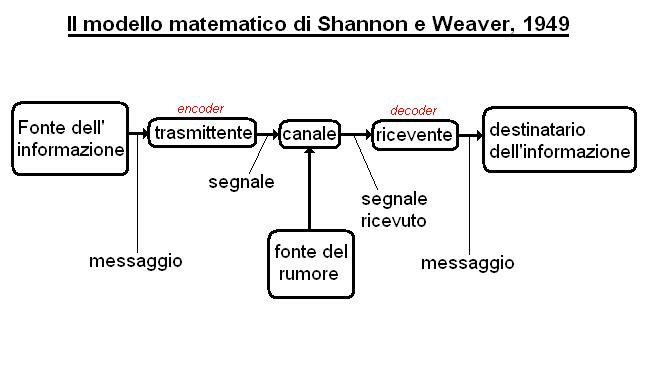
\includegraphics[width=\linewidth]{img/communication-model.jpg}
    \caption{Modello della comunicazione.}
    \label{fig:communication-model}
\end{figure}

La comunicazione è strutturata in cinque fasi:
\begin{enumerate}
    \item codifica di sorgente: il mittente rimuove la ridondanza dal messaggio.
    Di fatto, il messaggio viene compresso in maniera loss-less.
    \item codifica di canale: il mittente aggiunge ridondanza mirata al messaggio
    compresso, in modo da permettere al destinatario di rilevare e correggere
    eventuali errori presenti nel messaggio ricevuto.
    La codifica di canale è fondamentale in quanto, a seguito della
    codifica di sorgente, i bit del messaggio compresso assumono un'importanza
    maggiore rispetto a quelli del messaggio di partenza, in quanto sono
    in numero ridotto rispetto ad essi, ma trasportano la stessa quantità di
    informazione. La perdita o modifica di uno di questi bit, quindi,
    porterebbe a importanti modifiche nell'informazione trasmessa e quindi
    a una grave distorsione.
    \item trasmissione su canale, e quindi introduzione di errori nel messaggio,
    causati dal rumore.
    \item decodifica di canale: il destinatario verifica se il messaggio ricevuto
    è afflitto da errori, ed eventualmente li corregge.
    \item decodifica: il messaggio ricevuto e corretto viene decompresso,
    in modo che il destinatario ottenga il messaggio originale.
\end{enumerate}

Questi principi non sono del tutto estranei a fenomeni reali e "naturali":
il linguaggio umano, infatti, prevede che le parole più usate siano
molto spesso quelle più corte, e che il destinatario possa capire il senso
di una frase anche se alcune sue parole vadano perse, sia in una comunicazione
orale che in una comunicazione scritta.

La teoria dell'informazione può essere utilizzata anche in altri campi
diversi dalla comunicazione fisica su canale tra due entità: ad esempio,
essa permette di modellare correttamente l'evoluzione, nel corso del tempo,
di un messaggio che si trova nello stesso posto, impresso su un mezzo fisico.
Un esempio può essere un uomo primitivo che incide una pietra: esso si comporta
come il mittente, che "invia" il messaggio sulla pietra, ovvero lo incide;
nel corso del tempo, però, il messaggio inciso viene modificato da fenomeni
naturali (rumore). Il destinatario è colui che osserva le incisioni dopo
moltissimi tempo, come ad esempio un archeologo.


\printbibliography

\end{document}
